\documentclass[12pt,a4paper]{article}
\usepackage{ctex}
\usepackage{amsmath,amscd,amsbsy,amssymb,latexsym,url,bm,amsthm}
\usepackage{epsfig,graphicx,subfigure}
\usepackage{enumitem,balance}
\usepackage{wrapfig}
\usepackage{mathrsfs, euscript}
\usepackage[usenames]{xcolor}
\usepackage{hyperref}
\usepackage[vlined,ruled,commentsnumbered,linesnumbered]{algorithm2e}
\usepackage{float}
\usepackage{array}
\usepackage{diagbox}
\usepackage{color}
\usepackage{indentfirst}
\usepackage{fancyhdr}
\usepackage{gensymb}
\usepackage{geometry}
\usepackage{setspace}
\usepackage{aurical}
\usepackage{times}
\usepackage{caption}
\usepackage{fontspec}
\usepackage{booktabs}
\usepackage{listings}
\usepackage{xcolor}
\setmainfont{Times New Roman}

\newtheorem{theorem}{Theorem}[section]
\newtheorem{lemma}[theorem]{Lemma}
\newtheorem{proposition}[theorem]{Proposition}
\newtheorem{corollary}[theorem]{Corollary}
\newtheorem{exercise}{Exercise}[section]
\newtheorem*{solution}{Solution}
\theoremstyle{definition}

\newcommand{\tabincell}[2]{\begin{tabular}{@{}#1@{}}#2\end{tabular}}
\newcommand{\postscript}[2]
 {\setlength{\epsfxsize}{#2\hsize}
  \centerline{\epsfbox{#1}}}

\renewcommand{\baselinestretch}{1.05}

\setlength{\oddsidemargin}{-0.365in}
\setlength{\evensidemargin}{-0.365in}
\setlength{\topmargin}{-0.3in}
\setlength{\headheight}{0in}
\setlength{\headsep}{0in}
\setlength{\textheight}{10.1in}
\setlength{\textwidth}{7in}
\makeatletter \renewenvironment{proof}[1][Proof] {\par\pushQED{\qed}\normalfont\topsep6\p@\@plus6\p@\relax\trivlist\item[\hskip\labelsep\bfseries#1\@addpunct{.}]\ignorespaces}{\popQED\endtrivlist\@endpefalse} \makeatother
\makeatletter
\renewenvironment{solution}[1][Solution] {\par\pushQED{\qed}\normalfont\topsep6\p@\@plus6\p@\relax\trivlist\item[\hskip\labelsep\bfseries#1\@addpunct{.}]\ignorespaces}{\popQED\endtrivlist\@endpefalse} \makeatother

\begin{document}
\noindent
%==========================================================
\noindent\framebox[\linewidth]{\shortstack[c]{
\Large{\emph{关联规则分析与}Apriori\emph{算法}}\vspace{1mm}\\
CS245 \quad 数据科学基础 \quad 陆朝俊 \vspace{1mm} \\
叶泽林 515030910468}}

\section{问题描述}

关联规则分析是数据挖掘中活跃的研究方法之一,其目的是在一个数据集中找出各项之间的关联关系(这种关系一般没有在数据中直接表示出来)。Apriori是关联规则分析中最常用也是最经典的挖掘频繁项集的算法,在本次作业中,我将实现Apriori算法,从交易数据集中发现频繁项集,并生成相应的关联规则。

\section{解决方案\protect\footnote{本次作业的主要代码实现可参见附录 \ref{apd:code}}}

\subsection{数据集的准备}

为验证Apriori算法实现的正确性,我根据一定的规则生成了一个交易数据集,数据集的每个实例代表一条交易记录,共100个实例。我将商品分为食品(bread、milk、apple、orange、beer)电器(TV、PC、phone、fridge、ele\_oven)和工具(scissors、stapler、plate、knife、glue)三类,各按照一定的出现及组合概率生成相应的商品交易记录,具体的参数设定可参见附录 \ref{apd:dataset}。

\vspace{0.01\linewidth}
我认为对于交易情况的分析,仅使用模拟生成的数据集难以取得真实的结果,因此我额外在Groceries数据集上执行了Apriori算法。Groceries数据集是内置于R语言的关联分析数据集,来源于某杂货店一个月的真实交易记录,包含9835条交易记录及169种商品。我将其从R语言包中提取出并重组为.csv格式,再使用Apriori算法进行分析。

\subsection{Apriori算法}

Apriori算法是最经典的挖掘频繁项集的算法,实现了在大数据集上可行的关联规则提取,其核心思想是\textbf{通过连接产生候选项与其支持度,然后通过剪枝生成频繁项集},步骤主要为:

\begin{enumerate}

\item 找出所有的频繁项集(支持度大于等于给定的阈值);

\item 由频繁项集产生强关联规则(经过上个步骤后满足给定的置信度阈值的规则)。

\end{enumerate}

为验证Apriori算法实现的正确性,我先使用蛮力算法在模拟交易数据集上运行一次,将结果与Apriori算法的结果进行比较。验证算法的正确性后,在Groceries数据集上我则直接使用Apriori算法进行分析。


\section{实验及结果}

\subsection{模拟数据集}

我将支持度和置信度的阈值分别设置为0.1及0.6,蛮力算法的运行结果为:

\begin{table}[H]
	\renewcommand\arraystretch{1.35}
	\caption{蛮力算法在模拟交易数据集下发现的频繁项集}
	\label{tab:baoli_sim_sup}
	\centering
	
	\begin{tabular}{c|c|c|c}
		\centering
		频繁项集 & 支持度 & 频繁项集 & 支持度 \\
		\hline
		scissors & 0.25 & apple & 0.18 \\
		beer & 0.22 & fridge & 0.25 \\
		ele\_oven & 0.26 & stapler & 0.30 \\
		phone & 0.22 & glue & 0.23 \\
		plate & 0.23 & scissors, knife & 0.15 \\
		PC & 0.22 & ele\_oven, TV & 0.17 \\
		TV & 0.29 & scissors, stapler & 0.15 \\
		bread & 0.19 & glue, stapler & 0.16 \\
		orange & 0.21 & stapler, plate & 0.15 \\
		knife & 0.27 & stapler, knife & 0.15 \\
		milk & 0.18 & & \\		
	\end{tabular}
\end{table}

\begin{table}[H]
	\renewcommand\arraystretch{1.35}
	\caption{蛮力算法在模拟交易数据集下发现的关联规则}
	\label{tab:baoli_sim_con}
	\centering
	
	\begin{tabular}{c|c}
		\centering
		关联规则 & 置信度 \\
		\hline
		glue --> stapler & 0.70 \\
		scissors --> knife & 0.60 \\
		ele\_oven --> TV & 0.65 \\
		plate --> stapler & 0.65 \\
		scissors --> stapler & 0.60 \\
	\end{tabular}
\end{table}

得到以上的参考结果后,我使用自己实现的Apriori算法和同样的参数(支持度0.1,置信度0.6)对模拟交易数据集进行分析,所得结果见表 \ref{tab:apriori_sim_sup} 和表 \ref{tab:apriori_sim_con}。

\begin{table}[H]
	\renewcommand\arraystretch{1.35}
	\caption{Apriori算法在模拟交易数据集下发现的关联规则(按置信度排序)}
	\label{tab:apriori_sim_con}
	\centering
	
	\begin{tabular}{c|c}
		\centering
		关联规则 & 置信度 \\
		\hline
		scissors --> stapler & 0.60 \\
		scissors --> knife & 0.60 \\
		plate --> stapler & 0.65 \\
		ele\_oven --> TV & 0.65 \\
		glue --> stapler & 0.70 \\
	\end{tabular}
\end{table}

\begin{table}[H]
	\renewcommand\arraystretch{1.35}
	\caption{Apriori算法在模拟交易数据集下发现的频繁项集(按支持度排序)}
	\label{tab:apriori_sim_sup}
	\centering
	
	\begin{tabular}{c|c|c|c}
		\centering
		频繁项集 & 支持度 & 频繁项集 & 支持度 \\
		\hline
		stapler, scissors & 0.15 & PC & 0.22 \\
		knife, scissors & 0.15 & phone & 0.22 \\
		stapler, knife & 0.15 & glue & 0.23 \\
		plate, stapler & 0.15 &plate & 0.23 \\
		stapler, glue & 0.16 & scissors & 0.25 \\
		ele\_oven, TV & 0.17 & fridge & 0.25 \\
		milk & 0.18 & ele\_oven & 0.26 \\
		apple & 0.18 & knife & 0.27 \\
		bread & 0.19 & TV & 0.29 \\
		orange & 0.21 & stapler & 0.30 \\
		beer & 0.22 & & \\		
	\end{tabular}
\end{table}

将表 \ref{tab:baoli_sim_sup}, \ref{tab:baoli_sim_con}的结果排序后与上表对比,容易发现二者一致。考虑到模拟交易数据集在生成时的随机性,这个结果可以证明我实现的Apriori算法的正确性。

根据理论分析,Apriori算法相对于蛮力算法有着极大的效率优势,为探索这种优势,我在不同支持度下运行两种算法进行频繁项集挖掘,对比消耗的时间,结果参见 \ref{fig:time_com}。

\begin{figure}[H]
	\centering
	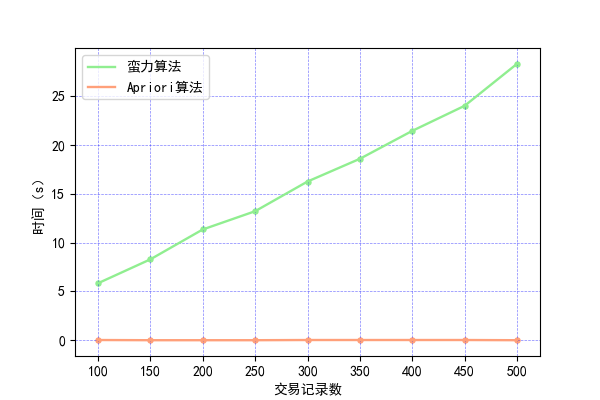
\includegraphics[width=0.7\linewidth]{img/time_kline.png}
	\caption{Apriori算法与蛮力算法进行频繁项集挖掘效率对比}
	\label{fig:time_com}
\end{figure}

从图中可以看出,相比于蛮力算法,Apriori算法具有极大的效率优势,上图的比较仅改变了数据集的交易记录数量,若增加总交易货品种类,蛮力算法的复杂度将呈指数型增长,Apriori算法的效率优势将更加明显。

\subsection{Groceries数据集}

确认Apriori算法实现的正确性后,我将其应用到真实数据上。考虑到Groceries数据集商品种类相对于实例较多的特点,每种商品出现的次数占总交易记录的比例可能偏低,因此我选择了较小的支持度(0.05),置信度选择为0.2。运行结果参见表 \ref{tab:apriori_gro_sup} 和表 \ref{tab:apriori_gro_con}。

\begin{table}[H]
	\renewcommand\arraystretch{1.35}
	\caption{Apriori算法在Groceries数据集下发现的频繁项集(按支持度排序)}
	\label{tab:apriori_gro_sup}
	\centering
	
	\begin{tabular}{c|c|c|c}
		\centering
		频繁项集 & 支持度 & 频繁项集 & 支持度 \\
		\hline
		napkins & 0.05 & canned beer & 0.08 \\
		beef & 0.05 & newspapers & 0.08 \\
		curd & 0.05 & bottled beer & 0.08 \\
		butter & 0.06 & citrus fruit & 0.08 \\
		yogurt, whole milk & 0.06 & pastry & 0.09 \\
		rolls/buns, whole milk & 0.06 & sausage & 0.09 \\
		pork & 0.06 & shopping bags & 0.10 \\
		coffee & 0.06 & tropical fruit & 0.10 \\
		margarine & 0.06 & root vegetables & 0.11 \\
		frankfurter & 0.06 & bottled water & 0.11 \\
		domestic eggs & 0.06 & yogurt & 0.14 \\
		brown bread & 0.06 & soda & 0.17 \\
		whipped/sour cream & 0.07 & rolls/buns & 0.18 \\
		fruit/vegetable juice & 0.07 & other vegetables & 0.19 \\
		other vegetables, whole milk & 0.07 & whole milk & 0.26 \\
		pip fruit & 0.08 & &
	\end{tabular}
\end{table}

\begin{table}[H]
	\renewcommand\arraystretch{1.35}
	\caption{Apriori算法在Groceries数据集下发现的关联规则(按置信度排序)}
	\label{tab:apriori_gro_con}
	\centering
	
	\begin{tabular}{c|c}
		\centering
		关联规则 & 置信度 \\
		\hline
		whole milk --> yogurt & 0.22 \\
		whole milk --> rolls/buns & 0.22 \\
		whole milk --> other vegetables & 0.29 \\
		rolls/buns --> whole milk & 0.31 \\
		other vegetables --> whole milk & 0.39 \\
		yogurt --> whole milk & 0.40 \\
	\end{tabular}
\end{table}

结果表明,频繁项集集中在大小为1或2的集合中。为进一步利用Apriori算法探索Groceries数据集的关联规则,我尝试了不同的支持度和置信度,具体结果可参见图 \ref{fig:apriori}。

%\vspace{-0.012\linewidth}
\begin{figure}[H]
	\centering
	\subfigure[频繁项集个数]{
		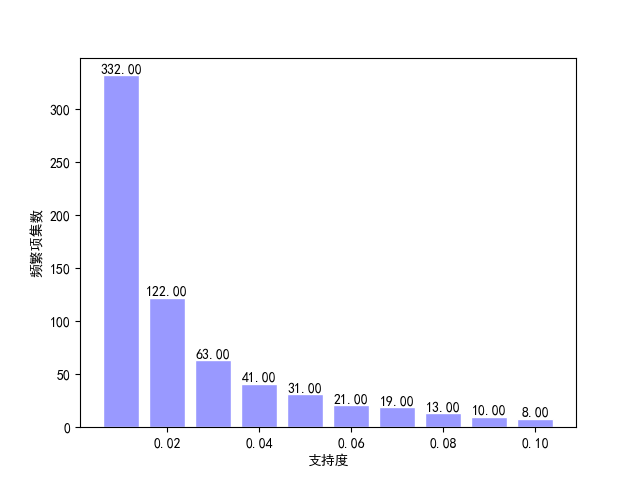
\includegraphics[width=0.45\linewidth]{img/gro_item_bar.png}
	}
	\subfigure[关联规则个数]{
		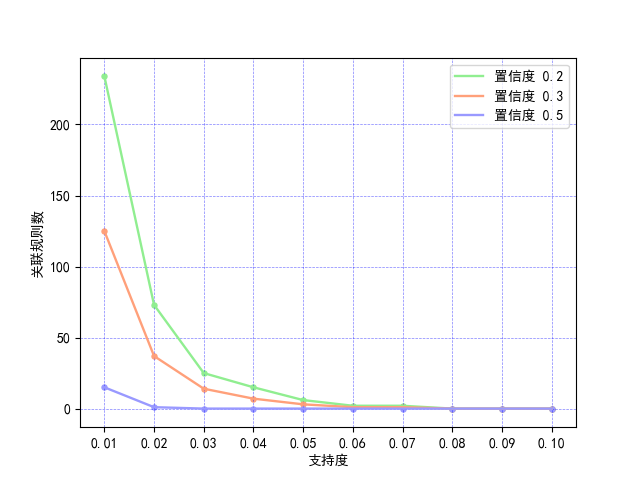
\includegraphics[width=0.45\linewidth]{img/gro_rule_kline.png}
	}
	\caption{频繁项集个数及关联规则个数与支持度和置信度关系}
	\label{fig:apriori}
\end{figure}

结果表明,在支持度大于0.1时,Groceries数据集中基本已找不出满足条件的频繁项集;而置信度大于0.5时,几乎无法在剩余的频繁项集中发现关联规则。这个结果进一步证明了实验前的假设:每种商品出现的次数占总交易记录的比例偏低。同时,从置信度和关联规则个数的关系分析,Groceries数据集中的交易记录存在一定的关联规则,但相应的置信度普遍偏低(0.5以下)。

\section{结论}

本次作业中,我利用Python语言实现了Apriori算法,并通过在模拟交易数据集上和蛮力算法的结果比较,证明了实现的正确性。之后我使用Apriori算法对模拟交易数据集以及Groceries数据集进行了频繁项集挖掘,进而分析关联规则。结果表明,Apriori算法是迅速且有效的挖掘频繁项集的算法,在中小规模的数据集上有着良好的表现(限于计算资源,我没有进行大规模数据上的实验)。

\newpage
\begin{appendix}
	\section{附录}
	\subsection{模拟交易数据集的详细信息}
	\label{apd:dataset}
	
	我将模拟交易数据集的交易记录按照交易商品数分为4类,即2、3、4、5件。不同的商品件数按照不同的比例随机混合三类商品,具体混合规则可参见表 \ref{tab:dataset}。
	
	\begin{table}[H]
		\renewcommand\arraystretch{1.35}
		\caption{模拟交易数据集生成交易记录的混合规则}
		\label{tab:dataset}
		\centering
		
		\begin{tabular}{c|c}
			\centering
			商品数 & 混合规则(括号中数字代表各类商品在记录中所占数量) \\
			\hline
			2 & (2); (1, 1) \\
			3 & (3); (2, 1) \\
			4 & (4); (3, 1); (2, 1, 1) \\
			5 & (5); (4, 1); (3, 2); (2, 2, 1) \\		
		\end{tabular}
	\end{table}
	
	
	\subsection{Apriori算法实现代码}
	\label{apd:code}
	
	\begin{lstlisting}[language=Python,
	numbers=left,
	keywordstyle=\color{blue!70},
	frame=shadowbox,
	breaklines=True]
from itertools import chain, combinations
from collections import defaultdict

class Apriori(object):
    def __init__(self, f_name, sup=0.1, con=0.1):
        self.data = self._read_csv(f_name)
        self.sup = sup
        self.con = con
        self.items = []
        self.rules = []

    def _read_csv(self, f_name):
        with open(f_name, 'r') as f:
            for line in f:
                line = line.strip().rstrip(',')
                item = frozenset(line.split(','))
                yield item

    def run(self):
        # 小工具函数
        def _get_support(item):
            return float(freq_set[item]) / len(deals)
        def _get_subsets(item):
            return chain(*[combinations(item, i + 1) for i, a in enumerate(item)])
        def _join_set(item_set, length):
            return set([i.union(j) for i in item_set for j in item_set if len(i.union(j)) == length])

        # 初始化 L1 项集和交易数据
        item_set, deals = self._init_data()

        freq_set = defaultdict(int)
        large_set = dict()

        init_set = self._remove_item_set(item_set, deals, freq_set)
        l_set = init_set

        k = 2
        while (l_set != set([])):
            large_set[k - 1] = l_set
            l_set = _join_set(l_set, k)
            c_set = self._remove_item_set(l_set, deals, freq_set)
            l_set = c_set
            k += 1

        # 组合结果
        for key, value in large_set.items():
            self.items.extend([(tuple(item), _get_support(item)) for item in value])

        for key, value in list(large_set.items())[1:]:
            for item in value:
                _subsets = map(frozenset, [x for x in _get_subsets(item)])
                for element in _subsets:
                    remain = item.difference(element)
                    if len(remain) > 0:
                        con = _get_support(item) / _get_support(element)
                        if con >= self.con:
                            self.rules.append(((tuple(element), tuple(remain)), con))

    def _init_data(self):
        deal_list = list()
        item_set = set()

        for d in self.data:
            deal = frozenset(d)
            deal_list.append(deal)

            # 产生 L1 项集
            for item in deal:
                item_set.add(frozenset([item]))

        return item_set, deal_list

    # 根据支持度阈值删除项集
    def _remove_item_set(self, item_set, deals, freq_set):
        res = set()
        local_set = defaultdict(int)

        # 统计
        for item in item_set:
            for d in deals:
                if item.issubset(d):
                    freq_set[item] += 1
                    local_set[item] += 1

        # 删除
        for item, count in local_set.items():
            support = float(count) / len(deals)
            if support >= self.sup:
                res.add(item)

        return res

    # 输出结果
    def show(self):
        print(u'------频繁项集------')
        for item, sup in sorted(self.items, key=lambda items: items[1]):
            print ('%s , %.2f' % (str(item), sup))
        print (u'\n------关联规则------')
        for rule, con in sorted(self.rules, key=lambda rules: rules[1]):
            pre, post = rule
            print ('%s --> %s , %.2f' % (str(pre), str(post), con))

if __name__ == "__main__":
    a = Apriori('groceries.csv', 0.05, 0.2)
    a.run()
    a.show()
	\end{lstlisting}
	
\end{appendix}

%========================================================================
\end{document}